\section{Desarrollo experimental 5}

Ahora pasaremos a usar un amplificador operacional el cual será posible usarlo en tanto a lazo abierto como en lazo cerrado, además de poder variar las resistencias de carga.\\
El esquema del mismo es el siguiente:

\begin{figure}[H]
    \centering
    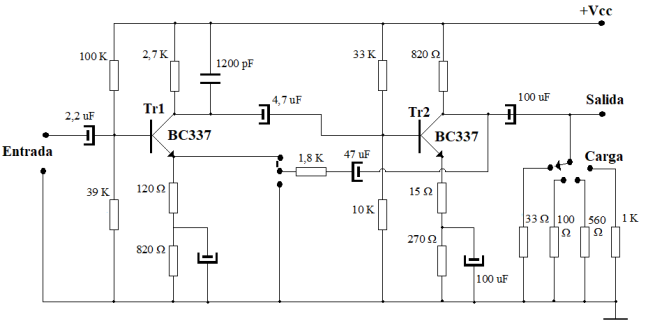
\includegraphics[width=0.5\textwidth]{images/esquema5.png}
    \caption{Conexiones realizadas}
    \label{fig:conexiones5}
\end{figure}

En la placa se verá de la siguiente forma:

\begin{figure}[H]
    \centering
    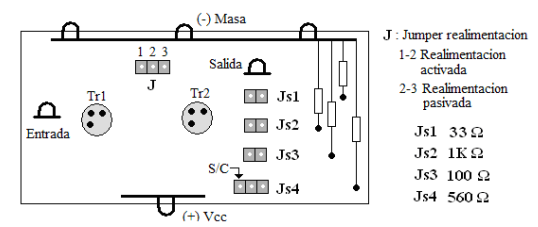
\includegraphics[width=0.5\textwidth]{images/esquema5b.png}
    \caption{Placa del amplificador operacional}
    \label{fig:placa5}
\end{figure}

Primero realizamos las mediciones a lazo abierto, por lo que conectamos J entre las terminales 2 y 3, y Js lo desconectamos.\\
Pondremos el generador a una frecuencia de 1KHz y una amplitud máxima sin distorsión.\\
Luego mediremos la señal de entrada y la señal de salida, y con esto podremos calcular la ganancia del amplificador operacional a lazo abierto.\\

\begin{figure}[H]
    \centering
    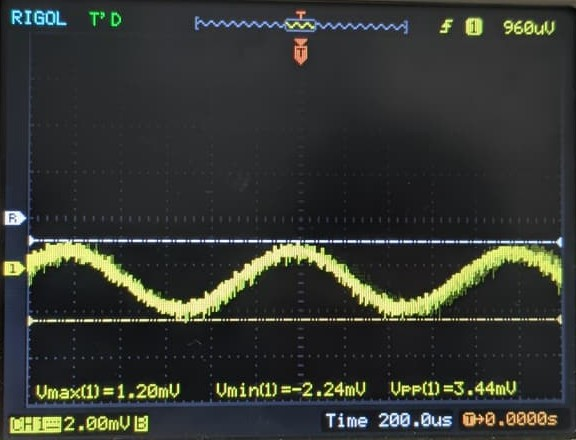
\includegraphics[width=0.4\textwidth]{images/punto5.jpeg}
    \caption{Medición de señal de entrada}
    \label{fig:entrada5}
\end{figure}

\begin{figure}[H]
    \centering
    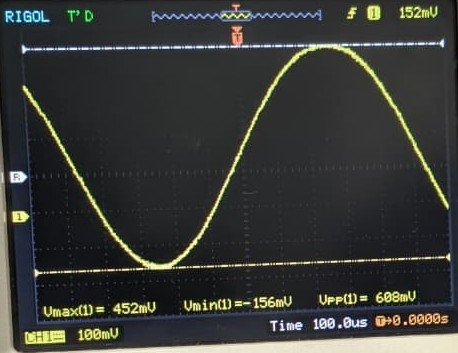
\includegraphics[width=0.4\textwidth]{images/punto5b.jpeg}
    \caption{Medición de señal de salida}
    \label{fig:salida5}
\end{figure}

\begin{table}[H]
\resizebox{\columnwidth}{!}{%
\begin{tabular}{|c|c|c|}
\hline
Vi (Vpap) & Vo (Vpap) & A=Vo/Vi \\ \hline
3.3mV         & 608mV         & 184.24       \\ \hline
\end{tabular}%
}
\end{table}

Ahora tal y como esta conectamos Js para la carga Rl = 1Kohm, y medimos nuevamente la señal de salida, y mediante calculo obtenemos Ro.\\

\begin{table}[H]
\resizebox{\columnwidth}{!}{%
\begin{tabular}{|c|c|c|}
\hline
Vo (Vpap) & Vs (Vpap) & Ro=Rl(Vo/Vs - 1) \\ \hline
608mV         & 390mV         & 558.97       \\ \hline
\end{tabular}%
}
\end{table}

Luego pasamos a retirar Js y cerramos el lazo, nuevamente buscamos la amplitud máxima sin distorsión y medimos la señal de entrada y salida para obtener la ganancia a lazo cerrado.\\

\begin{figure}[H]
    \centering
    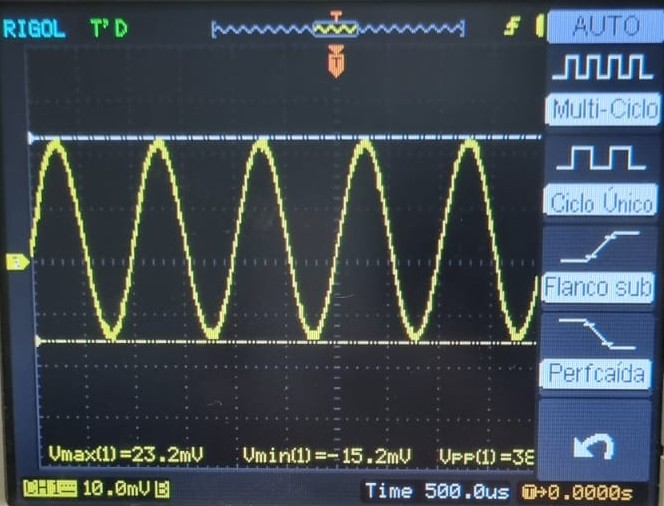
\includegraphics[width=0.4\textwidth]{images/punto5c.jpeg}
    \caption{Medición de señal de entrada a lazo cerrado}
    \label{fig:entrada5c}
\end{figure}

\begin{table}[H]
\resizebox{\columnwidth}{!}{%
\begin{tabular}{|c|c|c|}
\hline
Vi (Vpap) & Vo’ (Vpap) & G=Vo’/Vi \\ \hline
3.3mV         & 37.5mV         & 11.36       \\ \hline
\end{tabular}%
}
\end{table}

Ahora calcularemos Ro’:

\begin{equation*}
Ro’ =\frac{Ro \cdot G}{A}
\end{equation*}

\begin{equation*}
Ro’ = 34.4\ \Omega
\end{equation*}

Para comprobar este valor haremos las mismas mediciones que en la 2da parte pero con el amplificador operacional a lazo cerrado, y calcularemos Ro’ mediante la formula de la parte 2.

\begin{figure}[H]
    \centering
    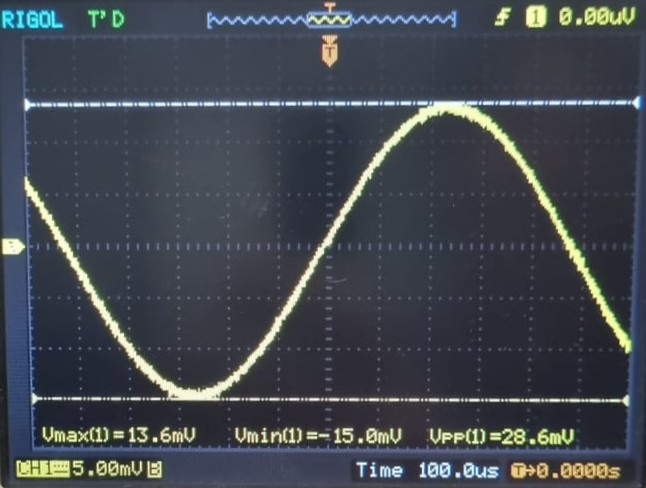
\includegraphics[width=0.4\textwidth]{images/punto5d.jpeg}
    \caption{Medición de señal de salida a lazo cerrado}
    \label{fig:salida5d}
\end{figure}

\begin{table}[H]
\resizebox{\columnwidth}{!}{%
\begin{tabular}{|c|c|c|}
\hline
Vo’ (Vpap) & Vs’ (Vpap) & Ro’=Rl(Vo/Vs - 1) \\ \hline
37.5mV         & 28.6mV         & $31.12\Omega$       \\ \hline
\end{tabular}%
}
\end{table}

\section{Desarrollo Experimental 6}

Para este experimento mediremos la potencia máxima de salida para lazo abierto, para ello ajustaremos el amplificador al mínimo, conectaremos Rc1 el cua deberá tener un valor cercano a lo calculado en la segunda parte, este valor será 550 $\Omega$, aumentamos la amplitud de la señal de entrada hasta que la señal de salida se distorsione, y medimos la potencia máxima de salida.\\

\begin{figure}[H]
    \centering
    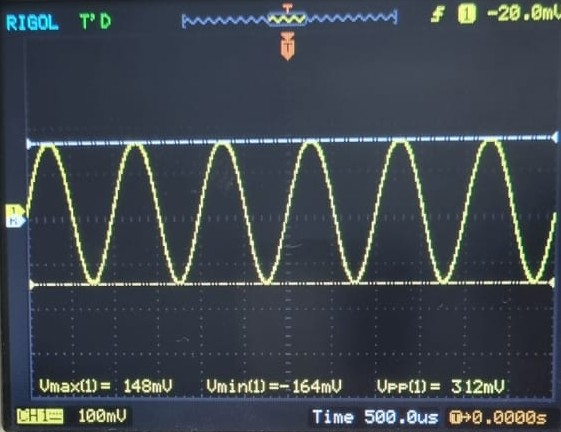
\includegraphics[width=0.4\textwidth]{images/punto6.jpeg}
    \caption{Medición de señal de salida a lazo abierto}
    \label{fig:salida6}
\end{figure}

Con este dato pasamos a calcular la potencia máxima de salida:
\begin{equation*}
Pmax = \frac{Vo^2}{8 \cdot Rc1}
\end{equation*}
\begin{equation*}
Pmax = 0.022mW
\end{equation*}

Luego pasamos a cerrar el lazo y repetimos el mismo procedimiento para medir la potencia máxima de salida a lazo cerrado.\\

\begin{figure}[H]
    \centering
    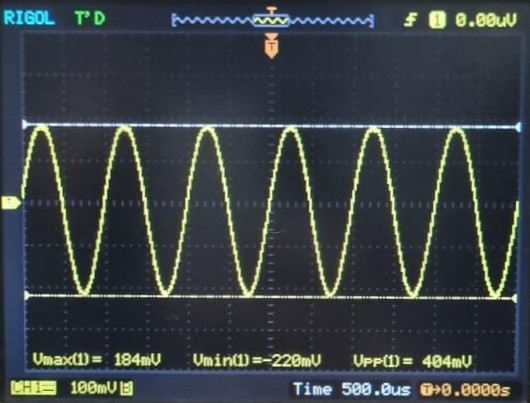
\includegraphics[width=0.4\textwidth]{images/punto6b.jpeg}
    \caption{Medición de señal de salida a lazo cerrado}
    \label{fig:salida6b}    
\end{figure}

Y calculamos la potencia máxima de salida a lazo cerrado:
\begin{equation*}
Pmax = \frac{Vo^2}{8 \cdot Rc1}
\end{equation*}
\begin{equation*}
Pmax = 0.62mW
\end{equation*}

